
\section{Related \lsystem generators}

In this section are listed other computer programs or web pages that allows to process \lsystems and eventually interpret them in most cases as an image.

\subsection{Web based}
\label{sec:WebBasedGenerators}

\subsubsection{\lsystem generator by Michael Norris}
\srcurl{http://www.michaelnorris.info/software/l-system-generator.html}

\noindent
Simple script which offers to set basic properties of \lsystem namely number of iterations, axiom and up to 15 rewrite rules.
Result is list of strings of symbols from all iterations (it does not interpret symbols).

This site can be used to familiarize with rewriting principles of \lsystems but it offers no additional functionality.


\subsubsection{Lindenmayer power by MadFlame Software}
\srcurl{http://madflame991.blogspot.com/p/lindenmayer-power.html}

\noindent
\lsystem generator which offers to set basic properties of \lsystem and interpretation for each symbol.
Symbols can be interpreted as turtle graphics or they can define or modify value of variable.
All iterations are listed as text and drawn on screen as well.

Possibility to work with variables makes it relatively powerful system but it is possible to draw only with thin black line.
Also syntax not very user-friendly and user interface is hard to use (and script it is not very stable).
Output window in only $500 \times 500$ pixels and it can not be saved otherwise than using print-screen.


\subsubsection{\lsystem generator by Nolan Carroll}	
\srcurl{http://nolandc.com/sandbox/fractals/}

\noindent
\lsystem generator with nice looking interface where is possible to set basic properties of \lsystem.
Symbols interpretation is fixed.
Last iteration of \lsystem is drawn on the screen using animation (line by line from start position).

Interface is user friendly but only drawable interpretation of symbol is black line.
There is no help nor examples thus it is hard to use for inexperienced user.
Output is drawn on canvas which fills entire area of web browser but it can not be saved otherwise than using print-screen.


\subsubsection{VRML \lsystem generator by Patrick Murris}
\srcurl{http://www.alpix.com/vrml/lsys.htm}
  
\noindent
\lsystem generator which can generate 3D VRML model.
Basic properties of \lsystem and interpretation can be set and output can be produced into VRML 1.0, 2.0 or string.

The problem is that VRML plugin is needed for displaying 3D models.



\subsubsection{\lsystem generator by John Snyders}
\srcurl{http://hardlikesoftware.com/projects/lsystem/lsystem.html}

\noindent
At first sight it is sophisticated \lsystem generator which can rewrite symbols with parameters and do context-sensitive rewriting.
Result is drawn on page as animation of development and progress bar shows its status.
The biggest drawback is that \lsystems are hard-coded in JavaScript and it is only possible to browse them in different iterations.

This \lsystem generator contains many examples and output is rendered as image which can be saved but examples are the only thing what it can produce.


\subsubsection{WWW \lsystem Explorer by Zdík Kudrle}
\srcurl{http://zdeeck.borg.cz/wlse/l-system.php}

\begin{wrapfigure}{r}{0.45\textwidth}
	\vspace{-20pt}
	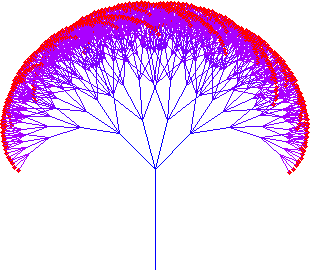
\includegraphics[width=\linewidth]{WwwLsystemExplorer}
	\caption{Image produced by WWW \lsystem Explorer}
	\label{fig:lsysExplorer}
\end{wrapfigure}

\noindent
\lsystem generator with well-arranged user interface where is possible to set basic properties of generated \lsystem.
Symbols interpretation is fixed and it uses unusual set of interpretation methods like \emph{pen up} and \emph{pen down} instead o traditional \emph{draw line} and \emph{move forward}.
The last iteration is drawn as an image by server-side PHP script thus output can be downloaded easily.
It is possible to set line color (even to color gradient) and background color of image.
Size of output image can be set freely.

This web-based generator is the best among the generators listed in this section.
It contains well written help section and few examples.
However it can not do context rewriting and symbols can not hold any parameters.
The length of drawn lines or turns can be affected only by increasing \emph{depth level} and setting the change ratio.
Example of plantlike model produced by WWW \lsystem Explorer is in \autoref{fig:lsysExplorer}.




\subsection{Desktop applications}
\label{sec:DesktopGenerators}

\subsubsection{\lsystems explorer by James Matthews}
\label{sec:LsystemExplorer}
\srcurl{http://www.generation5.org/content/2002/lse.asp}

\noindent
Simple desktop application which renders \lsystems in the application window.
Basic properties of \lsystem and its interpretation can be edited in dialog window but interpretation for individual symbols can not be changed.
It is possible to move and zoom model with mouse.
\lsystems can be saved or loaded into text file and drawn image can be saved to clipboard.

\lsystems explorer can be used for generation of simple models but it is not possible to do context rewriting of use symbols parameters.
Even line thickness can not be changed.
User interface for editing \lsystem is very simple (it is possible to show rewrite rules only for one symbol at a time).


\subsubsection{\lsystem Vector Generator by Dmitry Malutin}
\srcurl{http://xaraxtv.at.tut.by/lsvg.htm}

\begin{wrapfigure}{r}{0.4\textwidth}
	\vspace{-20pt}
	
\includegraphics[width=\linewidth]{LsystemVectorGenerator}
	\caption{Plant example from \lsystem Vector Generator}
	\label{fig:lsvg}
\end{wrapfigure}

\noindent
Similar application to \nameref{sec:LsystemExplorer} but with better user interface and it is also possible to randomize line lengths or turn angles.
Nice feature is \emph{angle wizard} which displays grid \lsystems each with different setting of turn angle and you can pick what you like.
Drawn lines drawn can be automatically closed to form polygons.
It is possible to save image as AI (Adobe Illustrator) or WMF (Windows Metafile) which are not very common formats.

Application contains hundreds of examples but it lack any advanced types of \lsystems or interpretation settings.
Application window size is about $700 \times 550$ pixels and it can not be resided.
One of built-in examples with randomized angles and line lengths is in \autoref{fig:lsvg}.


\subsubsection{\lsystem 4 by Timothy Perz}
\srcurl{http://www.oocities.org/tperz/L4About.htm}

\noindent
\lsystem 4 is relatively advanced tool for generating models with \lsystems.
Besides all basic functionality it is possible to create 3D models with custom textures.
Models can be saved to raster images as BMP or JPEG or they can be exported to AutoCAD DXF format.
Interpreting capabilities are quite good but \lsystem rewriting can do only deterministic rewriting with limited usage of parameters.

Table of symbols interpretations (which are not changeable) can be displayed at right side of application which is nice feature.
\lsystem 4 have good capabilities in producing 3D output but the input syntax is very compact and hard to read.
Also more advanced \lsystem types like context-sensitive or parametric \lsystems are not supported.

\newcommand{\lstudio}{\mbox{L-studio}\xspace}

\subsubsection{\lstudio by Przemysław Prusinkiewicz et. al}
\srcurl{http://algorithmicbotany.org/lstudio/}

\noindent
\lstudio is probably one of the best applications designed for modeling plants with \lsystems.
\lstudio is not single program but it is complex solution that consists of many tools.
\lstudio can process all types of \lsystems described in \autoref{sec:lsysTypes} and also it can produce animation of plant growth.
With \lstudio is possible to model 3D models of plants with regards to environment like wind, gravity, space the around plant, sun light, etc.
Output can be saved in many formats like Wavefront OBJ, Postscript, BMP or render plant with built in ray-tracer to produce photo-realistic images.

Even there is many examples of plant models and extensive help it is not easy to start using it.
The syntax is very compact and quite unclear for new user.

Application is not free-ware but demo version can be downloaded.
After evaluation period it is still possible to use it but it is not possible to export images and previews have watermark.
In \autoref{fig:lstudio} is one of the most beautiful examples in \lstudio, the Lily.


\begin{figure}[h]
	\centering
	
\includegraphics[width=0.8\linewidth]{Lily}
	\caption{Model of Lily produced by \lstudio}
	\label{fig:lstudio}
\end{figure}





















